\section{IMO y OIM}

\subsection{Encuentro 1}

\begin{section-problem}
    Hallar todos los posibles números reales que satisfacen\footnote{$\lfloor x \rfloor$ representa la parte entera de $x$.}
    \[x\cdot\lfloor x \rfloor + 2022 = \lfloor x^2 \rfloor\]
\end{section-problem}

\begin{section-problem}
    Demuestre que para todo $n \geq 4$ existen enteros positivos distintos $a_1, a_2, \cdots, a_n$ para los cuales se cumple que
    \[\frac{20}{21} = \inverseOf{a_1} + \inverseOf{a_2} + \cdots + \inverseOf{a_n}.\]
\end{section-problem}

\begin{section-problem}
    Decimos que un conjunto $S$, posiblemente infinito, de enteros positivos distintos es bueno si para cualesquieras par de elementos $m, n \in S$, con $m \neq n$, se tiene que la diferencia $|m - n|$ divide a $m$ y $n$, simultáneamente.
    \begin{enumerate}
        \item Demuestra que un conjunto bueno no puede tener una cantidad infinita de elementos.
        \item Demuestra que para todo entero positivo $N \geq 2$, existe un conjunto bueno con $N$ elementos.
    \end{enumerate}
\end{section-problem}

\begin{section-problem}
    En un tablero de $n \times n$, el conjunto de todas las casillas que están ubicadas en la diagonal principal del tablero o debajo de ella, es llamado \textit{n-escalera}.
    Por ejemplo, en la siguiente figura se muestra una \textit{3-escalera}:
    \begin{figure}[htb]
        \centering
        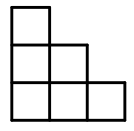
\includegraphics[width=1.4cm]{images/3-escalera}
    \end{figure}
    
    ¿De cuántas formas se puede dividir una \textit{99-escalera} en algunos rectángulos, que tengan sus lados sobre líneas de la cuadrícula, de tal forma que todos los rectángulos tengas áreas distintas?
\end{section-problem}

\begin{section-problem}
    Encontrar todas las funciones inyectivas $f: \N \rightarrow \N$, tales que satisfacen $f(1) = 2$, $f(2) = 4$ y
    \[f(f(m) + f(n)) =  f(f(m)) + f(n).\]
\end{section-problem}

\begin{section-problem}
    Sea $n > 2$, un entero y $P(x)$ un polinomio de coeficientes reales tal que para un real $k$
    \begin{gather*}
        \frac{P(2) - P(1)}{1} = \frac{P(4) - P(2)}{2} =\\
        \frac{P(8) - P(4)}{4} = \cdots = \frac{P(2^n) - P(2^{n - 1})}{2^{n - 1}} = k \\
        \\
        \frac{P(2^{n + 1}) - P(2^n)}{2^n} \neq k
    \end{gather*}
    Hallar el valor mínimo del grado de $P$ y todos los posibles polinomios $P$ con grado mínimo.
\end{section-problem}

\begin{section-problem}
    Sean $a$, $b$, $c \in \R^+$, tal que $a + b + c = 0$.
    Demostrar que
    \[\sqrt[n]{ab + bc + ca} \geq a \sqrt[n]{\frac{b + c}{2}} + b \sqrt[n]{\frac{c + a}{2}} + c \sqrt[n]{\frac{a + b}{2}}.\]
\end{section-problem}

\begin{section-problem}
    Sea
    \[\frac{r}{s} = 0. k_1 k_2 k_3 \cdots\]
    la expansión decimal de un número racional.
    Probar que a lo más dos de los números
    \begin{gather*}
        \sigma_1 = 10 \left(\frac{r}{s}\right) - k_1, \quad
        \sigma_2 = 10^2 \left(\frac{r}{s}\right) - (10 k_1 + k_2),\\
        \sigma_3 = 10^3 \left(\frac{r}{s}\right) - (10^2 k_1 + 10 k_2 + k_3), \quad \cdots
    \end{gather*}
    son iguales.

\end{section-problem}


\subsection{Encuentro 2}

\begin{section-problem}
    Encuentra todas las funciones $f: \Z \rightarrow \Z$ tales que para cualesquiera enteros $m$, $n$ tenemos
    \[f(m + n) + f(mn - 1) = f(m)f(n).\]
\end{section-problem}

\begin{section-problem}
    Encontrar todas las fuciones $f: \N \rightarrow \N$ que para todo $x,y \in N$ se cumple que
    \[f(x + y) = f(x) + f(y) + 3(x + y)\sqrt[3]{f(x)f(y)}.\]
\end{section-problem}

\begin{section-problem}
    Encontrar todas las funciones $f$ tal que
    \[f(f(x) + y) = f(x^2 - y) + 4yf(x)\]
    para todo real $x$ y $y$.
\end{section-problem}

\begin{section-problem}
    Determinar todos los enteros $n \geq 2$ que tengan la siguiente propiedad:
    para cualquier entero $a_1$, $a_2$, $\cdots$, $a_n$ cuya suma no sea divisible por $n$, existe un índice $1 \leq i \leq n$ tal que ninguno de los números
    \[a_i, a_i + a_{i + 1}, \cdots, a_i + a_{i + 1} + \cdots + a_{i + n - 1}\]
    es divisible por $n$.
    Aquí, dejamos $a_i = a_{i - n}$ cuando $i > n$.
\end{section-problem}

\begin{section-problem}
    Sea $n$ un entero impar.
    Pintaremos los vértices de un n-ágono regular con tres colores talque hay un número impar de vértices de cada color.
    Probar que existen un triángulo isósceles con los tres vértices de diferente color.
\end{section-problem}

\begin{section-problem}
    Determinar todas las funciones $f: \Z \rightarrow \Z$ con la propiedad
    \[f(x - f(y)) = f(f(x)) - f(y) - 1\]
    para todo entero $x, y \in \Z$.
\end{section-problem}

\begin{section-problem}
    Sea ${a_i}_{n}$ una sucesión de reales positivos que satisface
    \[a_{k + 1} \geq \frac{k a_k}{a_k^2 + (k - 1)}\]
    para todo entero positivo $k$.
    Muestra que $a_1 + a_2 + \cdots + a_n \geq n$, para todo $n \geq 2$.
\end{section-problem}

\begin{section-problem}
    Encuentre todas las funciones $f: \R^{+} \rightarrow \R^{+}$ que satisfacen
    \[x^2(f(x) + f(y)) = (x + y)f(yf(x)).\]
\end{section-problem}

